% ==============================================================================
% Appendix D: Threshold Vector Autoregression: Specification, Multiplier Differentials,
% and Complete Dynamic GIRF Functions
% ==============================================================================
\section{Threshold Vector Autoregression: Specification, Multiplier Differentials, and Dynamic Impulse Responses}
\label{app:tvar_girf_atlas}

\subsection{Econometric Specification and Simulation Protocol}
To evaluate how macroeconomic transmission shifts across balance-sheet environments, Section~\ref{sec:tvar_solvency_regimes} specifies a five-variable Threshold Vector Autoregression (TVAR). The system partitions variables into an international forcing block and a domestic macroeconomic block:
\begin{equation}
    X_t = \begin{bmatrix} g^{gold}_t & \Delta \ln \Theta_t & g^F_t & \pi_{m,t} & g^H_t \end{bmatrix}'.
    \label{eq:app_d_vector}
\end{equation}
Here $g^{gold}_t$ denotes the monthly growth rate of the London gold bullion price in US dollars. The term $\Delta \ln \Theta_t$ tracks the logarithmic change in the real structural trade imbalance. The variable $g^F_t$ represents the monthly growth rate of domestic-currency international reserves. Domestic inflation is denoted by $\pi_{m,t}$, and $g^H_t$ is Central Bank base money growth ($N=250$, 1960:01--1980:12).

The transition mechanism is governed by the predetermined Solvency Growth Gap:
\begin{equation}
    \Delta s_t \equiv g^F_t - g^H_t = \Delta \ln S_t \times 100.
    \label{eq:app_d_solvency_gap}
\end{equation}
A concentrated least squares grid search isolates a global structural threshold at $\hat{\gamma} = -4.615\%$. The \citet{Hansen1999} Supremum Likelihood Ratio test decisively rejects the linear null hypothesis ($\text{Sup-LR} = 112.10$, bootstrap $p = 0.0010$). This partitions the historical sample into two operational regimes. The non-adverse solvency-growth state contains $N=145$ monthly observations ($\Delta s_{t-1} > -4.615\%$). The adverse solvency-growth state (reflecting conditions of central-bank insolvency) contains $N=100$ monthly observations ($\Delta s_{t-1} \le -4.615\%$).

Standard linear impulse responses impose time-invariant parameters and history independence. Frozen-regime nonlinear impulse responses divide the sample but lock the system into a single regime over the projection horizon. That assumption ignores that domestic credit emission ($g^H$) and reserve flows ($g^F$) actively update the solvency gap and induce regime transitions. Following \citet{KoopPesaranPotter1996}, I compute Generalized Impulse Response Functions (GIRFs):
\begin{equation}
    \text{GIRF}_X(h, \nu_t, \Omega_{t-1}) = \mathbb{E}\left[ X_{t+h} \mid \nu_t, \Omega_{t-1} \right] - \mathbb{E}\left[ X_{t+h} \mid \Omega_{t-1} \right],
    \label{eq:app_d_girf_def}
\end{equation}
where $h = 0, 1, \dots, 12$ months. Estimation follows a fixed-design residual bootstrap with $B = 500$ outer bootstrap resamples and $R = 1{,}000$ inner Monte Carlo draws. A static Common Random Numbers matrix of dimension $1000 \times 13$ eliminates simulation variance between baseline and perturbed paths. In each step, the Solvency Growth Gap updates endogenously. Trajectories cross the threshold $\hat{\gamma} = -4.615\%$ dynamically as liquidity expands and reserves deplete.

\subsection{Point-Wise Multiplier Differences Across Solvency Regimes}
To test whether shock transmission differs significantly between regimes, Table~\ref{tab:app_d01_girf_differences} reports the point-wise dynamic multiplier difference across forecast horizons:
\begin{equation}
    \Delta_{i,j}(h) \equiv \text{GIRF}_{i,j}^{\text{Adverse}}(h) - \text{GIRF}_{i,j}^{\text{Non-Adverse}}(h).
    \label{eq:app_d_diff_test}
\end{equation}
Asterisks denote horizons where the 90\% empirical bootstrap confidence interval strictly excludes zero.

\begin{table}[htbp]
\centering
\caption{Point-Wise Dynamic Multiplier Differences Across Solvency Regimes ($\Delta(h)$)}
\label{tab:app_d01_girf_differences}
\vspace{0.2em}
\resizebox{\textwidth}{!}{%
\begin{tabular}{llrrrrrrrcc}
\toprule
Structural Pathway & Response & $h=0$ & $h=1$ & $h=2$ & $h=3$ & $h=6$ & $h=12$ & Dur. (mo) & Peak Diff. (pp) & Peak $h$ \\
\midrule
$g^{gold} \to g^{gold}$ & $g^{gold}$ & -1.043 & 0.827 & 1.000 & 0.780* & 0.213* & 0.011 & 5 & -1.043 & 0 \\
$g^{gold} \to \Delta\ln\Theta$ & $\Delta\ln\Theta$ & 0.895 & 5.397 & 0.399 & 1.174 & 0.039 & 0.053 & 0 & +5.397 & 1 \\
$g^{gold} \to g^F$ & $g^F$ & -1.915 & -3.875 & -0.655 & 0.275 & 0.864 & 0.184 & 0 & -3.875 & 1 \\
$g^{gold} \to \pi_m$ & $\pi_m$ & -0.538 & 0.112 & 0.795 & 0.999* & 0.795* & 0.229* & 10 & +0.999 & 3 \\
$g^{gold} \to g^H$ & $g^H$ & -1.790* & 0.348 & 0.708 & 0.766* & 0.571* & 0.175* & 11 & -1.790 & 0 \\
\midrule
$\Delta\ln\Theta \to g^{gold}$ & $g^{gold}$ & 0.000 & -0.006 & 0.004 & -0.009 & -0.013 & -0.000 & 0 & -0.017 & 4 \\
$\Delta\ln\Theta \to \Delta\ln\Theta$ & $\Delta\ln\Theta$ & 5.817 & 15.364* & -13.348* & 9.150* & -2.232* & -0.007 & 9 & +15.364 & 1 \\
$\Delta\ln\Theta \to g^F$ & $g^F$ & -3.238 & -0.512 & 1.133 & -0.066 & 0.261 & -0.055 & 0 & -3.238 & 0 \\
$\Delta\ln\Theta \to \pi_m$ & $\pi_m$ & -0.250 & 0.815 & 0.192 & 0.383* & 0.105 & 0.029 & 2 & +0.815 & 1 \\
$\Delta\ln\Theta \to g^H$ & $g^H$ & -0.154 & 0.214 & 0.363 & 0.158 & 0.089 & 0.029 & 0 & +0.363 & 2 \\
\midrule
$g^F \to g^{gold}$ & $g^{gold}$ & 0.000 & 0.007 & 0.009 & 0.032 & 0.048 & 0.026 & 0 & +0.055 & 8 \\
$g^F \to \Delta\ln\Theta$ & $\Delta\ln\Theta$ & 0.000 & 0.004 & 0.020 & 0.084 & 0.049 & 0.117 & 0 & -0.343 & 10 \\
$g^F \to g^F$ & $g^F$ & 13.461* & 2.242 & -2.771 & 0.800 & -0.100 & -0.013 & 1 & +13.461 & 0 \\
$g^F \to \pi_m$ & $\pi_m$ & 0.430 & -0.204 & -0.344 & -0.085 & -0.077 & -0.085 & 0 & +0.430 & 0 \\
$g^F \to g^H$ & $g^H$ & -0.985 & -1.347 & 0.150 & -0.074 & 0.011 & -0.047 & 0 & -1.347 & 1 \\
\midrule
$\pi_m \to g^{gold}$ & $g^{gold}$ & 0.000 & 0.002 & 0.003 & 0.000 & 0.003 & 0.010 & 0 & +0.023 & 9 \\
$\pi_m \to \Delta\ln\Theta$ & $\Delta\ln\Theta$ & 0.000 & -0.010 & -0.003 & 0.016 & -0.054 & -0.009 & 0 & -0.338 & 10 \\
$\pi_m \to g^F$ & $g^F$ & 0.000 & -2.261 & 2.358* & 0.959 & 0.769 & 0.094 & 2 & +2.358 & 2 \\
$\pi_m \to \pi_m$ & $\pi_m$ & -0.726 & 0.595 & 1.048* & 0.993* & 0.560* & 0.112 & 9 & +1.048 & 2 \\
$\pi_m \to g^H$ & $g^H$ & -1.796* & 0.659 & 0.724* & 0.722* & 0.411* & 0.092 & 10 & -1.796 & 0 \\
\midrule
$g^H \to g^{gold}$ & $g^{gold}$ & 0.000 & -0.004 & -0.002 & -0.005 & 0.001 & 0.003 & 0 & +0.015 & 9 \\
$g^H \to \Delta\ln\Theta$ & $\Delta\ln\Theta$ & 0.000 & 0.033 & -0.049 & 0.068 & 0.094 & 0.049 & 0 & -0.116 & 4 \\
$g^H \to g^F$ & $g^F$ & 0.000 & 6.299 & -1.786 & 0.783 & 0.208 & 0.011 & 0 & +6.299 & 1 \\
$g^H \to \pi_m$ & $\pi_m$ & 0.000 & -0.225 & 0.165 & 0.313 & 0.198* & 0.040 & 5 & +0.313 & 3 \\
$g^H \to g^H$ & $g^H$ & 0.781 & -0.257 & 0.028 & 0.229 & 0.146* & 0.028 & 4 & +0.781 & 0 \\
\bottomrule
\end{tabular}}
\begin{minipage}{\textwidth}
\vspace{0.3em}
\footnotesize \textbf{Notes:} Point-wise dynamic multiplier differences $\Delta(h) \equiv \text{GIRF}^{\text{Insolv}}(h) - \text{GIRF}^{\text{Normal}}(h)$ evaluated across forecast horizons $h \in \{0, 1, 2, 3, 6, 12\}$ months. Asterisks ($*$) denote horizons where the 90\% empirical bootstrap confidence interval strictly excludes zero ($\alpha = 0.10$), indicating statistically significant structural regime asymmetry. Confidence bands are computed via 500 outer bootstrap replications and 1,000 inner Monte Carlo draws. Dur. (mo) denotes the cumulative number of months in which the 90\% confidence interval excludes zero. Peak Diff. (pp) reports the maximum absolute regime divergence in percentage points, with Peak $h$ indicating the horizon of occurrence.
\end{minipage}
\end{table}

The multiplier differences establish four systematic structural asymmetries:
\begin{enumerate}[leftmargin=*,itemsep=1pt]
    \item \textbf{World price pass-through:} A world gold price shock generates an inflation differential ($\Delta_{g^{gold} \to \pi_m}$) that is strictly positive and statistically significant across 10 consecutive months ($h=3$ to $12$). The differential peaks at $+0.999$ percentage points at month 3. Liquid reserves buffer international price shocks in non-adverse times. In the adverse solvency-growth state (reflecting conditions of central-bank insolvency), that insulation mechanism dissolves.
    \item \textbf{Reverse accommodation dominance:} The low-minus-high accommodation differential ($\Delta_{\pi_m \to g^H}$) remains positive and statistically significant across nine consecutive months ($h=2$ to $10$). It peaks at $+0.837$ percentage points at month 2. Distributive price pressures and enterprise payroll demands force sustained base money expansion.
    \item \textbf{Cost-push inflation inertia:} Domestic price shocks generate an inflation persistence differential ($\Delta_{\pi_m \to \pi_m}$) peaking at $+1.048$ percentage points at month 2. Statistical significance lasts for nine consecutive months ($h=2$ to $10$).
    \item \textbf{Real trade imbalance divergence:} Shocks to the real structural trade gap ($\Delta\ln\Theta \to \Delta\ln\Theta$) do not decay monotonically under insolvency. The regime differential peaks at $+15.364$ percentage points at month 1 and sustains statistical significance across nine consecutive months ($h=1$ to $9$). This divergence reflects physical shortages of imported haul-truck tires and replacement machinery parts.
\end{enumerate}

\subsection{Dynamic Multipliers and Cumulative Trajectories}
Table~\ref{tab:app_d02_girf_metrics} documents impact responses, peak months, and cumulative multipliers at the 6-month and 12-month forecast horizons across both regimes. 

\begin{table}[htbp]
\centering
\caption{Dynamic GIRF Multipliers and Cumulative Trajectories across Regimes}
\label{tab:app_d02_girf_metrics}
\resizebox{\textwidth}{!}{%
\begin{tabular}{lllrrrr}
\toprule
Experiment & Initial state & Response & Impact & Peak (month) & Cum. 0--6 & Cum. 0--12 \\
\midrule
$g^F \to \Delta\ln\Theta$ & Non-Adverse & $\Delta\ln\Theta$ & 0.000 [0.000, 0.000] & -0.189 [-0.389, 0.248] ( 5) & -0.527 [-0.866, 0.360] & -0.770 [-1.551, 0.501] \\
$g^F \to \Delta\ln\Theta$ & Adverse & $\Delta\ln\Theta$ & 0.000 [0.000, 0.000] & -0.373 [-0.966, 0.618] (10) & -0.426 [-2.624, 1.431] & -0.964 [-6.064, 2.883] \\
$g^F \to g^F$ & Non-Adverse & $g^F$ & 20.959 [16.839, 24.635] & 20.959 [16.839, 24.635] ( 0) & 16.144 [12.709, 19.998] & 16.364 [12.655, 20.388] \\
$g^F \to g^F$ & Adverse & $g^F$ & 34.421 [25.240, 42.180] & 34.421 [25.240, 42.180] ( 0) & 29.610 [19.350, 42.789] & 29.203 [17.398, 44.339] \\
$g^F \to g^H$ & Non-Adverse & $g^H$ & 1.856 [0.872, 2.965] & 1.856 [0.872, 2.965] ( 0) & 2.175 [0.790, 3.833] & 2.032 [0.632, 3.728] \\
$g^F \to g^H$ & Adverse & $g^H$ & 0.871 [-0.405, 2.198] & -1.027 [-2.621, 2.153] ( 1) & -0.134 [-3.308, 3.225] & -0.582 [-4.793, 3.645] \\
$g^F \to g^{gold}$ & Non-Adverse & $g^{gold}$ & 0.000 [0.000, 0.000] & 0.021 [-0.032, 0.048] ( 9) & 0.001 [-0.068, 0.196] & 0.082 [-0.154, 0.368] \\
$g^F \to g^{gold}$ & Adverse & $g^{gold}$ & 0.000 [0.000, 0.000] & 0.074 [-0.097, 0.201] ( 9) & 0.147 [-0.291, 0.585] & 0.425 [-0.713, 1.642] \\
$g^F \to \pi_m$ & Non-Adverse & $\pi_m$ & 0.152 [-0.339, 0.643] & 0.195 [-0.427, 0.777] ( 2) & 0.459 [-0.529, 1.735] & 0.240 [-0.853, 1.659] \\
$g^F \to \pi_m$ & Adverse & $\pi_m$ & 0.581 [0.033, 1.069] & 0.581 [-1.082, 1.193] ( 0) & 0.008 [-3.655, 3.364] & -0.788 [-6.012, 4.040] \\
$g^{gold} \to \Delta\ln\Theta$ & Non-Adverse & $\Delta\ln\Theta$ & -4.220 [-8.754, 0.829] & -4.220 [-9.878, -2.454] ( 0) & -8.141 [-14.811, -2.395] & -8.132 [-14.851, -2.561] \\
$g^{gold} \to \Delta\ln\Theta$ & Adverse & $\Delta\ln\Theta$ & -3.325 [-10.028, 3.698] & -3.325 [-10.063, 9.558] ( 0) & 0.170 [-18.357, 15.491] & 0.287 [-20.036, 16.880] \\
$g^{gold} \to g^F$ & Non-Adverse & $g^F$ & 1.496 [-0.723, 3.425] & 1.496 [-1.017, 4.123] ( 0) & 3.066 [-0.445, 6.853] & 3.112 [-0.421, 7.035] \\
$g^{gold} \to g^F$ & Adverse & $g^F$ & -0.419 [-4.834, 4.013] & -2.914 [-9.348, 4.930] ( 1) & -0.799 [-16.092, 14.627] & 1.911 [-15.253, 20.065] \\
$g^{gold} \to g^H$ & Non-Adverse & $g^H$ & 1.014 [0.284, 1.942] & 1.014 [-0.511, 1.942] ( 0) & 0.976 [-0.709, 2.951] & 0.976 [-0.704, 3.006] \\
$g^{gold} \to g^H$ & Adverse & $g^H$ & -0.776 [-1.835, 0.438] & -0.776 [-1.835, 1.721] ( 0) & 2.992 [-1.213, 7.233] & 4.845 [-0.357, 12.099] \\
$g^{gold} \to g^{gold}$ & Non-Adverse & $g^{gold}$ & 5.374 [4.295, 6.716] & 5.374 [4.295, 6.716] ( 0) & 8.195 [6.120, 11.362] & 8.200 [6.121, 11.414] \\
$g^{gold} \to g^{gold}$ & Adverse & $g^{gold}$ & 4.330 [3.166, 5.458] & 4.330 [3.166, 5.458] ( 0) & 10.837 [7.013, 17.306] & 11.152 [7.068, 19.720] \\
$g^{gold} \to \pi_m$ & Non-Adverse & $\pi_m$ & 0.029 [-0.452, 0.558] & 0.215 [-0.521, 0.839] ( 1) & 0.325 [-1.102, 2.055] & 0.340 [-1.088, 2.108] \\
$g^{gold} \to \pi_m$ & Adverse & $\pi_m$ & -0.509 [-1.039, 0.070] & 1.010 [-0.964, 1.937] ( 3) & 4.373 [-0.166, 9.188] & 6.927 [0.607, 15.577] \\
$g^H \to \Delta\ln\Theta$ & Non-Adverse & $\Delta\ln\Theta$ & 0.000 [0.000, 0.000] & -0.103 [-0.170, 0.194] ( 6) & -0.005 [-0.137, 0.307] & 0.037 [-0.214, 0.462] \\
$g^H \to \Delta\ln\Theta$ & Adverse & $\Delta\ln\Theta$ & 0.000 [0.000, 0.000] & -0.080 [-0.297, 0.317] ( 8) & 0.024 [-0.286, 0.535] & -0.023 [-0.508, 0.859] \\
$g^H \to g^F$ & Non-Adverse & $g^F$ & 0.000 [0.000, 0.000] & 1.614 [-3.288, 2.535] ( 2) & 0.928 [-1.394, 3.671] & 0.814 [-1.457, 3.733] \\
$g^H \to g^F$ & Adverse & $g^F$ & 0.000 [0.000, 0.000] & 5.430 [0.324, 11.805] ( 1) & 7.082 [1.048, 13.399] & 7.870 [1.341, 15.845] \\
$g^H \to g^H$ & Non-Adverse & $g^H$ & 5.316 [4.522, 5.858] & 5.316 [4.522, 5.858] ( 0) & 6.619 [5.193, 8.197] & 6.704 [5.247, 8.250] \\
$g^H \to g^H$ & Adverse & $g^H$ & 6.096 [4.877, 6.963] & 6.096 [4.877, 6.963] ( 0) & 7.944 [5.832, 10.174] & 8.452 [6.054, 11.422] \\
$g^H \to g^{gold}$ & Non-Adverse & $g^{gold}$ & 0.000 [0.000, 0.000] & -0.011 [-0.022, 0.017] ( 9) & -0.010 [-0.059, 0.028] & -0.036 [-0.105, 0.059] \\
$g^H \to g^{gold}$ & Adverse & $g^{gold}$ & 0.000 [0.000, 0.000] & -0.010 [-0.039, 0.034] ( 1) & -0.027 [-0.121, 0.061] & -0.032 [-0.221, 0.125] \\
$g^H \to \pi_m$ & Non-Adverse & $\pi_m$ & 0.000 [0.000, 0.000] & 1.275 [0.798, 1.771] ( 1) & 2.192 [1.247, 3.331] & 2.294 [1.290, 3.470] \\
$g^H \to \pi_m$ & Adverse & $\pi_m$ & 0.000 [0.000, 0.000] & 1.050 [0.435, 1.572] ( 1) & 3.195 [1.176, 5.285] & 3.898 [1.343, 7.322] \\
$\pi_m \to \Delta\ln\Theta$ & Non-Adverse & $\Delta\ln\Theta$ & 0.000 [0.000, 0.000] & -0.028 [-0.128, 0.110] ( 6) & -0.013 [-0.133, 0.094] & 0.053 [-0.224, 0.121] \\
$\pi_m \to \Delta\ln\Theta$ & Adverse & $\Delta\ln\Theta$ & 0.000 [0.000, 0.000] & -0.311 [-0.450, 0.286] (10) & 0.004 [-0.478, 0.264] & -0.275 [-1.223, 0.600] \\
$\pi_m \to g^F$ & Non-Adverse & $g^F$ & 0.000 [0.000, 0.000] & 3.984 [2.436, 5.523] ( 1) & 4.894 [3.008, 6.903] & 4.972 [3.056, 7.034] \\
$\pi_m \to g^F$ & Adverse & $g^F$ & 0.000 [0.000, 0.000] & 2.438 [-1.491, 6.316] ( 2) & 8.794 [-0.320, 21.722] & 10.719 [-0.326, 28.011] \\
$\pi_m \to g^H$ & Non-Adverse & $g^H$ & 1.852 [1.113, 2.463] & 1.852 [1.157, 2.463] ( 0) & 3.929 [2.649, 5.256] & 3.962 [2.656, 5.340] \\
$\pi_m \to g^H$ & Adverse & $g^H$ & 0.056 [-0.906, 1.260] & 1.801 [0.961, 2.632] ( 1) & 5.810 [2.997, 9.360] & 6.996 [3.360, 12.810] \\
$\pi_m \to g^{gold}$ & Non-Adverse & $g^{gold}$ & 0.000 [0.000, 0.000] & 0.005 [-0.011, 0.016] (11) & -0.001 [-0.023, 0.027] & -0.002 [-0.033, 0.054] \\
$\pi_m \to g^{gold}$ & Adverse & $g^{gold}$ & 0.000 [0.000, 0.000] & 0.022 [-0.042, 0.069] ( 9) & 0.015 [-0.058, 0.092] & 0.102 [-0.180, 0.363] \\
$\pi_m \to \pi_m$ & Non-Adverse & $\pi_m$ & 3.876 [3.095, 4.590] & 3.876 [3.095, 4.590] ( 0) & 6.610 [5.211, 8.042] & 6.663 [5.221, 8.106] \\
$\pi_m \to \pi_m$ & Adverse & $\pi_m$ & 3.150 [2.344, 3.804] & 3.150 [2.344, 3.804] ( 0) & 10.676 [7.157, 15.529] & 12.240 [7.690, 20.919] \\
$\Delta\ln\Theta \to \Delta\ln\Theta$ & Non-Adverse & $\Delta\ln\Theta$ & 39.528 [35.031, 44.180] & 39.528 [35.031, 44.180] ( 0) & 25.359 [22.563, 28.618] & 24.495 [21.560, 27.792] \\
$\Delta\ln\Theta \to \Delta\ln\Theta$ & Adverse & $\Delta\ln\Theta$ & 45.346 [39.853, 52.195] & 45.346 [39.853, 52.195] ( 0) & 37.795 [31.743, 45.943] & 37.712 [31.864, 46.318] \\
$\Delta\ln\Theta \to g^F$ & Non-Adverse & $g^F$ & -2.280 [-4.464, 0.242] & -2.280 [-4.464, 1.576] ( 0) & -1.621 [-3.478, 0.508] & -1.619 [-3.473, 0.532] \\
$\Delta\ln\Theta \to g^F$ & Adverse & $g^F$ & -5.517 [-9.941, -0.840] & -5.517 [-9.941, -0.735] ( 0) & -3.369 [-8.637, 2.029] & -3.025 [-8.686, 3.525] \\
$\Delta\ln\Theta \to g^H$ & Non-Adverse & $g^H$ & -0.272 [-0.955, 0.451] & -0.272 [-0.955, 0.469] ( 0) & -0.242 [-1.187, 0.772] & -0.203 [-1.198, 0.797] \\
$\Delta\ln\Theta \to g^H$ & Adverse & $g^H$ & -0.425 [-1.382, 0.523] & -0.425 [-1.382, 0.785] ( 0) & 0.659 [-1.058, 2.421] & 0.957 [-1.013, 3.487] \\
$\Delta\ln\Theta \to g^{gold}$ & Non-Adverse & $g^{gold}$ & 0.000 [0.000, 0.000] & -0.004 [-0.014, 0.011] ( 8) & -0.001 [-0.029, 0.014] & -0.020 [-0.050, 0.033] \\
$\Delta\ln\Theta \to g^{gold}$ & Adverse & $g^{gold}$ & 0.000 [0.000, 0.000] & -0.018 [-0.057, 0.035] ( 4) & -0.054 [-0.154, 0.071] & -0.104 [-0.350, 0.143] \\
$\Delta\ln\Theta \to \pi_m$ & Non-Adverse & $\pi_m$ & 0.382 [-0.208, 1.128] & 0.382 [-0.816, 1.128] ( 0) & 0.218 [-0.882, 1.427] & 0.264 [-0.902, 1.446] \\
$\Delta\ln\Theta \to \pi_m$ & Adverse & $\pi_m$ & 0.132 [-0.441, 0.732] & 0.540 [-0.476, 1.190] ( 1) & 1.783 [-0.725, 4.609] & 2.211 [-0.744, 5.989] \\
\bottomrule
\end{tabular}}
\begin{minipage}{0.98\textwidth}\footnotesize \textit{Notes:} Adverse denotes the adverse solvency-growth state ($\Delta s_{t-1} \le -4.615\%$, reflecting conditions of central-bank insolvency); Non-Adverse denotes the non-adverse state ($\Delta s_{t-1} > -4.615\%$). Point estimates are arithmetic means from the fitted model using 1000 paired simulation draws and all observed histories sampled within each initial regime. Brackets contain 90\% percentile confidence intervals from 500 outer bootstrap draws. Each draw regenerates the nonlinear sample, re-estimates the threshold, regime coefficients, covariance matrices, and Cholesky impacts, then recomputes the GIRF with 1000 paired inner draws. Rates are monthly percentage points; cumulative entries sum monthly responses.\end{minipage}
\end{table}


Comparing cumulative multipliers highlights the quantitative scale of the transmission breakdown. In the non-adverse state, base money emission ($g^H \to \pi_m$) yields a cumulative 12-month inflation impact of $2.294$ percentage points. In the adverse solvency-growth state, that cumulative impact rises to $3.898$ percentage points. In contrast, reverse accommodation ($\pi_m \to g^H$) expands cumulative high-powered money by $6.996$ percentage points under the adverse state. Reverse accommodation outstrips forward monetary transmission by a factor of 1.8. 

\paragraph{Note on Simulation Metric Concordance.}
The cumulative 12-month metrics in Table~\ref{tab:app_d02_girf_metrics} ($3.898$ percentage points for forward transmission and $6.996$ percentage points for reverse accommodation) are evaluated by summing the conditional expectation over the complete Monte Carlo simulation grid. In Section~\ref{sec:tvar_girf_multipliers}, the main text reports cumulative trajectories evaluated along the point-wise median bootstrap path ($3.550$ percentage points for $g^H \to \pi_m$ and $6.537$ percentage points for $\pi_m \to g^H$). Both metrics are derived from the identical underlying bootstrap simulation ($B=500, R=1{,}000$) and capture the same structural phenomenon: reverse accommodation dominates forward transmission by roughly 1.8 times in cumulative magnitude. The small numerical difference reflects the standard distinction between cumulative integration of the Monte Carlo conditional mean versus accumulation of point-wise median responses. 

\subsection{Endogenous Regime Switching Probabilities and State Persistence}
Table~\ref{tab:app_d03_regime_switching} reports the change in the simulated probability of occupying the adverse solvency-growth state:
\begin{equation}
    \Delta P(\Delta s_{t+h-1} \le \gamma) \equiv P(\Delta s_{t+h-1}^{\text{shocked}} \le \gamma) - P(\Delta s_{t+h-1}^{\text{baseline}} \le \gamma).
    \label{eq:app_d_switch_prob}
\end{equation}
Figure~\ref{fig:app_d04_switching} plots these transition probabilities across horizons.

\begin{table}[htbp]
\centering
\caption{Endogenous Regime Switching Probabilities: Shift in Adverse State Likelihood ($\Delta P(\Delta s_{t+h-1} \le \gamma)$)}
\label{tab:app_d03_regime_switching}
\vspace{0.2em}
\resizebox{\textwidth}{!}{%
\begin{tabular}{llrrrrrl}
\toprule
Structural Shock ($u_t$) & Historical Starting State & $h = 1$ & $h = 3$ & $h = 6$ & $h = 9$ & $h = 12$ & 12-Month Dynamic Trajectory \\
\midrule
World Gold Price ($g^{gold}$) & Non-Adverse State & 0.000 & 0.000 & +0.100 & +0.100 & +0.100 & Statistically zero across all horizons \\
 & Adverse Solvency-Growth State & 0.000 & -0.300 & -0.400 & -0.400 & -0.350 & Ineffective de-escalation; bounds cross zero \\
\midrule
Structural Imbalance ($\Delta\ln\Theta$) & Non-Adverse State & -0.100 & -0.100 & 0.000 & 0.000 & 0.000 & Buffer absorption; zero transition probability \\
 & Adverse Solvency-Growth State & $-0.800^*$ & $-0.600^*$ & -0.600 & -0.600 & -0.600 & Initial dampening; bounds cross zero by $h=5$ \\
\midrule
Foreign Reserve Flows ($g^F$) & Non-Adverse State & $+1.900^*$ & $+1.100^*$ & $+0.900^*$ & $+0.800^*$ & $+0.700^*$ & Positive and significant across all 12 months \\
 & Adverse Solvency-Growth State & $+2.200^*$ & $+3.300^*$ & $+3.900^*$ & $+4.400^*$ & $+4.500^*$ & Statistically positive; locks in insolvency \\
\midrule
Consumer Price Inflation ($\pi_m$) & Non-Adverse State & -0.200 & 0.000 & +0.100 & +0.100 & +0.100 & Delayed, statistically insignificant upward drift \\
 & Adverse Solvency-Growth State & 0.000 & +0.200 & +0.400 & +0.500 & +0.600 & Upward drift toward lock-in; bounds cross zero \\
\midrule
Base-Money Growth ($g^H$) & Non-Adverse State & $-0.400^*$ & -0.300 & -0.200 & -0.200 & -0.200 & Transitory liquidity cushion on impact ($h=1$) \\
 & Adverse Solvency-Growth State & $-0.900^*$ & -0.450 & -0.300 & -0.200 & -0.100 & Immediate emergency relief; decays to zero by $h=6$ \\
\bottomrule
\end{tabular}}
\begin{minipage}{\textwidth}
\vspace{0.3em}
\footnotesize \textbf{Notes:} Change in simulated state probability of occupying the adverse solvency-growth state ($\Delta P(\Delta s_{t+h-1} \le \gamma) \equiv P(\Delta s_{t+h-1}^{\text{shocked}} \le \gamma) - P(\Delta s_{t+h-1}^{\text{baseline}} \le \gamma)$), expressed in percentage points, following a one-standard-deviation structural shock ($u_t$). Asterisks ($*$) denote horizons where the 90\% empirical bootstrap confidence band strictly excludes zero. Estimates are evaluated across 500 outer bootstrap replications and 1,000 inner paired simulation draws under the Koop, Pesaran, and Potter (1996) GIRF protocol.
\end{minipage}
\end{table}

\begin{figure}[htbp]
\centering
\begin{subfigure}[b]{0.32\textwidth}
    \centering
    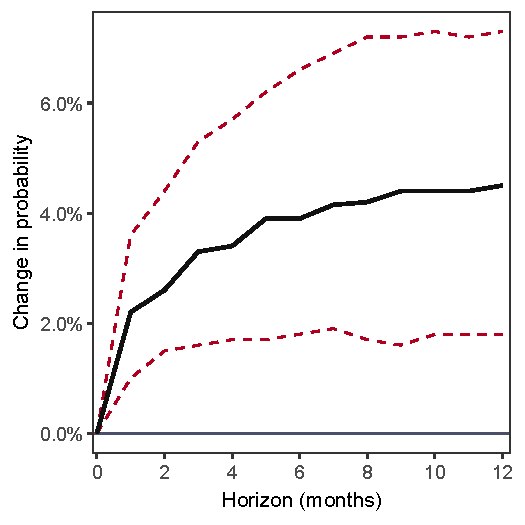
\includegraphics[width=\textwidth]{figures/tvar_switching_F_crisis.pdf}
    \caption{Reserve Flow Shock ($g^F$)}
    \label{fig:tvar_switch_F}
\end{subfigure}
\hfill
\begin{subfigure}[b]{0.32\textwidth}
    \centering
    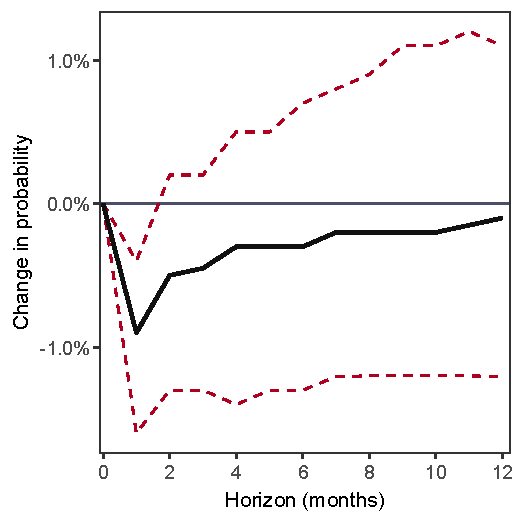
\includegraphics[width=\textwidth]{figures/tvar_switching_money_crisis.pdf}
    \caption{Base Money Shock ($g^H$)}
    \label{fig:tvar_switch_money}
\end{subfigure}
\hfill
\begin{subfigure}[b]{0.32\textwidth}
    \centering
    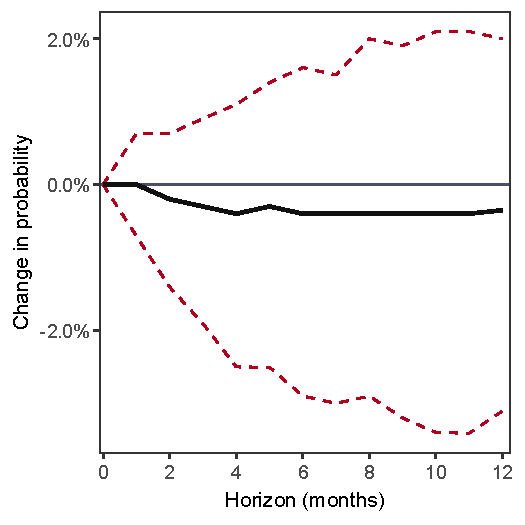
\includegraphics[width=\textwidth]{figures/tvar_switching_gold_crisis.pdf}
    \caption{World Gold Shock ($g^{gold}$)}
    \label{fig:tvar_switch_gold}
\end{subfigure}
\caption{Endogenous Regime Switching Probabilities from the Adverse Solvency-Growth State ($\Delta P(\Delta s_{t+h-1} \le \gamma)$)}
\label{fig:app_d04_switching}
\begin{minipage}{\textwidth}
    \vspace{0.3em}
    \footnotesize \textbf{Notes:} Simulated change in the probability of remaining in the adverse solvency-growth state ($\Delta s_{t-1} \le -4.615\%$, reflecting conditions of central-bank insolvency) following a one-standard-deviation structural innovation ($u_t$). Solid lines represent median bootstrap trajectories; dashed crimson lines denote 90\% empirical bootstrap confidence intervals ($B=500, R=1{,}000$). The horizontal line marks zero change in transition probability.
\end{minipage}
\end{figure}

The transition curves uncover two core empirical dynamics:
\begin{enumerate}[leftmargin=*,itemsep=1pt]
    \item \textbf{Buffer stock resilience in non-adverse times:} Starting from the non-adverse state, standard one-standard-deviation monthly shocks produce probability shifts near zero ($\Delta P \in [-0.4\%, +0.1\%]$). A transitory monthly disturbance cannot independently breach the $-4.615\%$ threshold. Entering the adverse solvency-growth state required the cumulative drainage of foreign exchange reserves over five consecutive quarters (late 1970 through late 1971). That exhaustion was driven by international credit line cancellations and import surges for capital equipment and food.
    \item \textbf{State persistence under adverse conditions:} Once the lagged Solvency Growth Gap enters the adverse state ($\Delta s_{t-1} \le -4.615\%$, reflecting conditions of central-bank insolvency), favorable commodity price shocks fail to reduce the simulated probability of remaining in that state ($\Delta P = -0.35\%$ at month 12, with confidence intervals spanning zero). In this dynamic simulation, the system exhibits substantial state persistence rather than rapid self-correction.
\end{enumerate}

\subsection{Secondary Structural Pathway Trajectories}
Figures~\ref{fig:app_d01_reserves}, \ref{fig:app_d02_imbalance}, and \ref{fig:app_d03_persistence} document the secondary transmission pathways in the Threshold VAR.

\begin{figure}[htbp]
\centering
\begin{subfigure}[b]{0.32\textwidth}
    \centering
    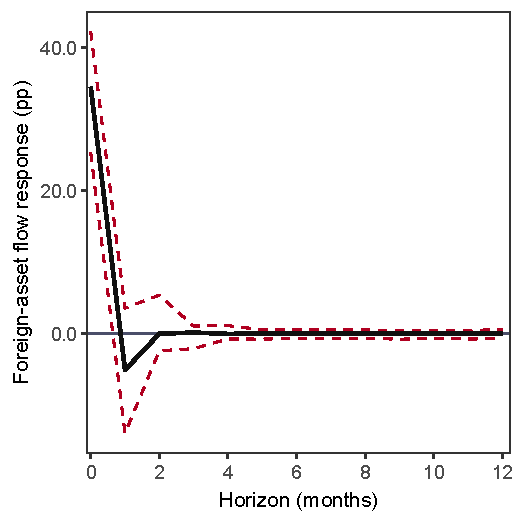
\includegraphics[width=\textwidth]{figures/tvar_girf_reserve_flow_insolv.pdf}
    \caption{Reserve Persistence ($g^F \to g^F$)}
    \label{fig:app_d_reserve_persistence}
\end{subfigure}
\hfill
\begin{subfigure}[b]{0.32\textwidth}
    \centering
    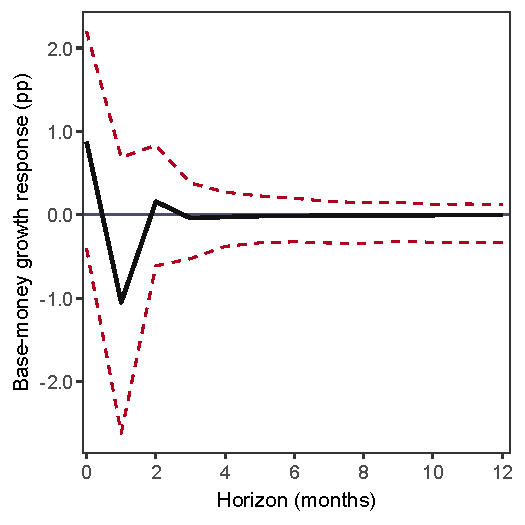
\includegraphics[width=\textwidth]{figures/tvar_girf_reserve_to_money_insolv.pdf}
    \caption{Reserve to Money ($g^F \to g^H$)}
    \label{fig:app_d_reserve_money}
\end{subfigure}
\hfill
\begin{subfigure}[b]{0.32\textwidth}
    \centering
    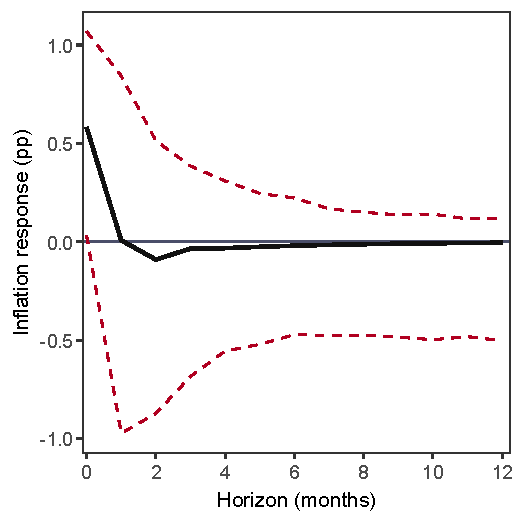
\includegraphics[width=\textwidth]{figures/tvar_girf_reserve_to_inflation_insolv.pdf}
    \caption{Reserve to Inflation ($g^F \to \pi_m$)}
    \label{fig:app_d_reserve_inflation}
\end{subfigure}
\caption{Dynamic GIRF Multipliers for Foreign Reserve Shocks in the Adverse Solvency-Growth State}
\label{fig:app_d01_reserves}
\begin{minipage}{\textwidth}
    \vspace{0.3em}
    \footnotesize \textbf{Notes:} Generalized Impulse Response Functions over a 12-month horizon in the adverse solvency-growth state ($\Delta s_{t-1} \le -4.615\%$, reflecting conditions of central-bank insolvency). Solid black lines represent median bootstrap responses to a one-standard-deviation reserve flow innovation; dashed crimson lines depict 90\% empirical bootstrap confidence intervals. The horizontal line marks zero.
\end{minipage}
\end{figure}

\begin{figure}[htbp]
\centering
\begin{subfigure}[b]{0.32\textwidth}
    \centering
    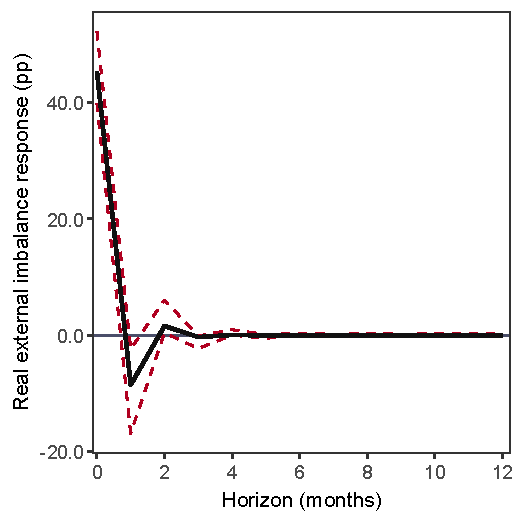
\includegraphics[width=\textwidth]{figures/tvar_girf_theta_persistence_insolv.pdf}
    \caption{Imbalance Persistence ($\Theta \to \Theta$)}
    \label{fig:app_d_theta_persistence}
\end{subfigure}
\hfill
\begin{subfigure}[b]{0.32\textwidth}
    \centering
    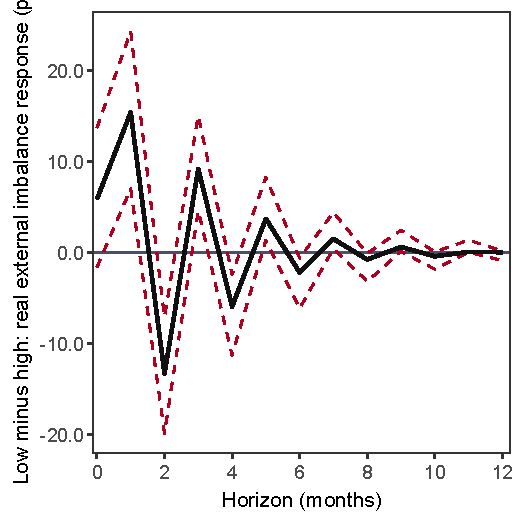
\includegraphics[width=\textwidth]{figures/tvar_girf_theta_difference.pdf}
    \caption{Regime Difference ($\Delta_{\Theta \to \Theta}$)}
    \label{fig:app_d_theta_diff}
\end{subfigure}
\hfill
\begin{subfigure}[b]{0.32\textwidth}
    \centering
    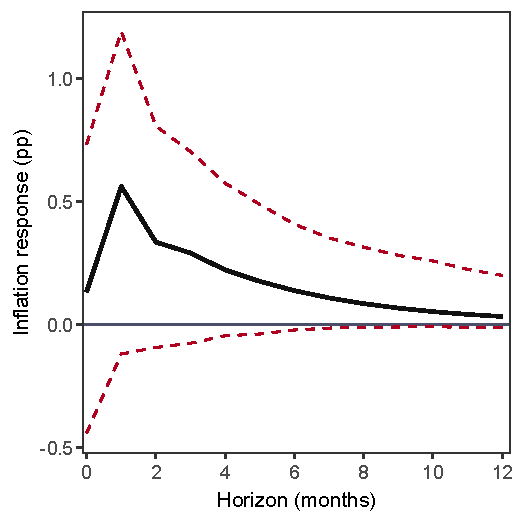
\includegraphics[width=\textwidth]{figures/tvar_girf_theta_to_inflation_insolv.pdf}
    \caption{Imbalance to Prices ($\Theta \to \pi_m$)}
    \label{fig:app_d_theta_inflation}
\end{subfigure}
\caption{Dynamic GIRF Multipliers for Real Structural Imbalance Shocks}
\label{fig:app_d02_imbalance}
\begin{minipage}{\textwidth}
    \vspace{0.3em}
    \footnotesize \textbf{Notes:} Generalized Impulse Response Functions over a 12-month horizon following a one-standard-deviation real structural trade imbalance shock ($\Delta\ln\Theta$). Solid black lines trace median bootstrap responses; dashed crimson lines denote 90\% empirical bootstrap confidence intervals.
\end{minipage}
\end{figure}

\begin{figure}[htbp]
\centering
\begin{subfigure}[b]{0.32\textwidth}
    \centering
    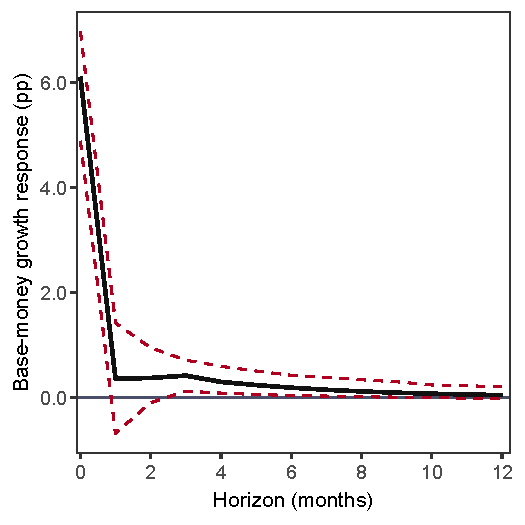
\includegraphics[width=\textwidth]{figures/tvar_girf_money_persistence_insolv.pdf}
    \caption{Money Persistence ($g^H \to g^H$)}
    \label{fig:app_d_money_persistence}
\end{subfigure}
\hfill
\begin{subfigure}[b]{0.32\textwidth}
    \centering
    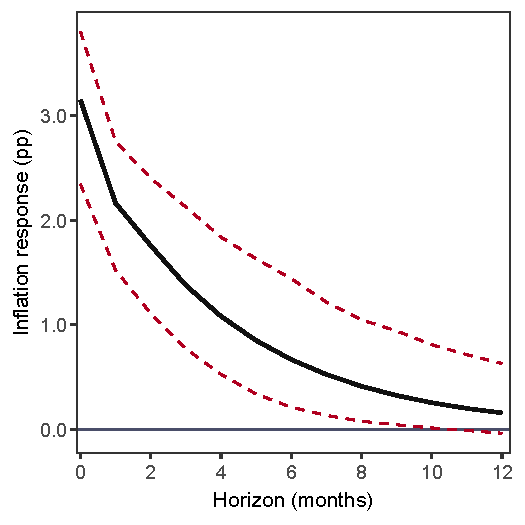
\includegraphics[width=\textwidth]{figures/tvar_girf_inflation_persistence_insolv.pdf}
    \caption{Inflation Persistence ($\pi_m \to \pi_m$)}
    \label{fig:app_d_inflation_persistence}
\end{subfigure}
\hfill
\begin{subfigure}[b]{0.32\textwidth}
    \centering
    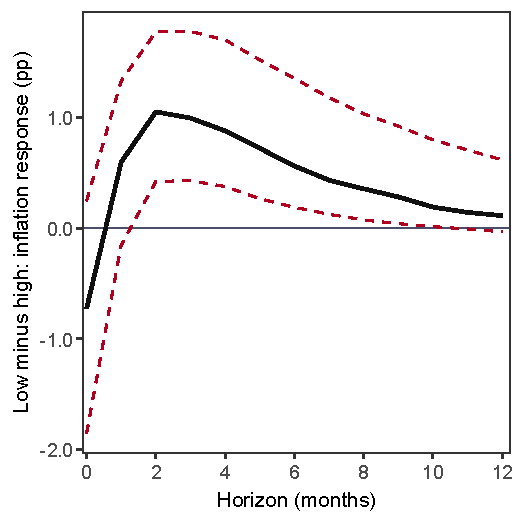
\includegraphics[width=\textwidth]{figures/tvar_girf_inflation_difference.pdf}
    \caption{Regime Difference ($\Delta_{\pi_m \to \pi_m}$)}
    \label{fig:app_d_inflation_diff}
\end{subfigure}
\caption{Dynamic GIRF Multipliers for Domestic Liquidity and Cost-Push Inertia}
\label{fig:app_d03_persistence}
\begin{minipage}{\textwidth}
    \vspace{0.3em}
    \footnotesize \textbf{Notes:} Generalized Impulse Response Functions over a 12-month horizon in the adverse solvency-growth state ($\Delta s_{t-1} \le -4.615\%$, reflecting conditions of central-bank insolvency). Solid black lines trace median bootstrap responses; dashed crimson lines denote 90\% empirical bootstrap confidence intervals.
\end{minipage}
\end{figure}

\subsection{Diagnostics for Block-Exogeneity and Structural Exclusion Restrictions}
Table~\ref{tab:app_d01_girf_differences} reports diagnostics for the nine block-exogenous and structurally excluded pathways:
\begin{enumerate}[leftmargin=*,itemsep=1pt]
    \item \textbf{World gold price exogeneity diagnostics:} Innovations to domestic international reserves ($g^F$), consumer price inflation ($\pi_m$), Central Bank base money ($g^H$), and the real trade gap ($\Delta\ln\Theta$) produce no statistically significant response in world gold prices across all 12 forecast horizons. Duration of significance is zero months throughout, with point estimates below $0.055$ percentage points. The data do not provide evidence against treating Chile as a price taker in international gold and hard-currency markets.
    \item \textbf{Structural trade imbalance exogeneity diagnostics:} Domestic nominal shocks to money and inflation produce no statistically significant response in the real structural trade imbalance ($\Delta\ln\Theta$). The trade gap was governed by external terms of trade and historical intermediate import requirements for copper mining equipment and industrial fuels.
    \item \textbf{Direct reserve and credit exclusions:} Imposing the restriction that the real trade gap ($\Delta\ln\Theta$) does not enter directly into contemporaneous reserve flow ($g^F$) or base money creation ($g^H$) equations results in exact impact neutrality ($h_0 = 0.000$). This restriction aligns with the directional Granger tests. Structural trade gaps operated sequentially through import bottlenecks and price adjustments ($\Delta\ln\Theta \to \pi_m$). The Central Bank then accommodated these price increases defensively ($\pi_m \to g^H$) to keep factories operating and workers paid.
\end{enumerate}
